\chapter{Curvas parametrizadas y longitud de un arco de curva}

\begin{ejercicio} Hallar una curva parametrizada $\alpha$ cuya traza es el círculo $x^2+y^2=1$, con $\alpha(t)$ recorriéndolo en el sentido de las agujas del reloj y con $\alpha(0) =(0,1)$.\\

Una solución a este ejercicio $\alpha(t)=(\sin t, \cos t)$. Es claro que $\alpha(0) =(\sin 0,\cos 0) =(0,1)$ y que al avanzar, por ejemplo a $\alpha(\frac{\pi}{2})=(\sin \frac{\pi}{2},\cos \frac{\pi}{2}) = (1,0)$ es en el sentido de las agujas del reloj.
\end{ejercicio}

\begin{ejercicio} Sea $\alpha(t)$  una curva que no pasa por el origen. Si $\alpha(t_0)$ es el punto de la traza de $\alpha$ más cercano al origen y $\alpha'(t_0)\neq 0$, demostrar que el vector posición $\alpha(t_0)$ es ortogonal a $\alpha'(t_0)$.\\

Definimos la función $D(t):=\alpha^2(t)=\alpha(t)\alpha(t)=\norm{\alpha(t)}^2$ que mide el cuadrado de la distancia de los puntos de la curva al origen.\\
$t_0$ es un punto relativo de dicha función por ser el punto más cercano al origen, entonces $D'(t_0)=0\implies 2\alpha(t_0)\alpha'(t_0)=0\implies\alpha(t_0)\perp\alpha'(t_0)$.
\end{ejercicio}

\begin{ejercicio} Sea $\ait$ una curva y $v\in\R^3$ un vector dado. Si $\alpha'(t)$ es ortogonal a $v$ para todo $t\in I$, y si $\alpha(0)$ también lo es, demuestre que $\alpha(t)$ es ortogonal a $v$ para todo $t\in I$.\\

Definimos $f(t):= \alpha(t)v= \alpha_1(t)v_1 + \alpha_2(t)v_2 +\alpha_3(t)v_3$.\\
Tenemos que $f'(t) = \alpha'(t)v= 0\ \forall t\in I$. Luego $f(t)= c\in \R,\ \forall t\in I$. Como en particular $f(0)=\alpha(0)v=0\implies c=0\implies \alpha(t)\perp v$.
\end{ejercicio}

\begin{ejercicio} Si $\ait$ es una curva regular, demuestre que $\norm{\alpha(t)}$ es constante (diferente de cero) si y sólo si $\alpha(t) \perp \alpha'(t)$ para todo $t\in I$.\\
\begin{itemize}
\item ($\implies$). $\norm{\alpha(t)}^2 = \alpha(t)\alpha(t)=c^2$. Derivando, $2\alpha(t)\alpha'(t)=0\implies \alpha(t)\perp\alpha'(t)$.
\item ($\impliedby$).$\alpha(t)\alpha'(t)=0\implies\dfrac{1}{2}(\alpha(t)\alpha(t))'=0\ximplies{\mathrm{Integrando}}{}\alpha(t)\alpha(t)=c\implies\\\implies\norm{\alpha(t)}^2=c\implies\norm{\alpha(t)}$ es constante.
\end{itemize}
\end{ejercicio}

\begin{ejercicio} Si $\ait$ es una curva, y $\function{M}{\R^3}{\R^3}$ es un movimiento rígido, demostrar que las longitudes de $\alpha$ y $M\circ\alpha$ entre $a\y b$ coinciden.\\

$\arc M\circ\alpha(t)=\integral{b}{a}\norm{(M\circ \alpha)'}=\integral{b}{a}\norm{M'(\alpha(s))\alpha'(s)}ds=\integral{b}{a}\norm{\overrightarrow{M}\alpha'(s)}ds\overset{\mathrm{por\ ser\ mov.\ rigido}}{=}\\=\integral{b}{a}\norm{\alpha'(s)}ds=\arc\alpha$.
\end{ejercicio}

\begin{ejercicio} Demuestre que las líneas tangentes a la curva $\alpha(t)=(3t,3t^2,2t^3)$ forman un ángulo constante con la recta $y=0,\ z=x$.\\

Tenemos que $\alpha'(t) = (3,6t,6t^2)$. La recta $r\equiv\doubleleft{y=0}{x=z}$ tiene como vector director\\$v:=(1,0,1)$. El ángulo $\theta$ que forman $v\y\alpha'(t)$ viene determinado por $\theta=\underset{[0,\pi)}\arccos\dfrac{\alpha'(t)v}{\norm{\alpha'(t)}\norm{v}}=\\=\underset{[0,\pi)}\arccos\dfrac{3+6t^2}{\sqrt{9+36t^2+36t^4}\sqrt{2}}=\underset{[0,\pi)}\arccos\dfrac{3+6t^2}{(3+6t^2)\sqrt{2}}=\underset{[0,\pi)}\arccos\dfrac{\sqrt{2}}{2}$ que es constante.
\end{ejercicio}
\begin{ejercicio} La curva engendrada por un punto $P$ de una circunferencia de radio $r$ que rueda sin
deslizar por una recta fija se llama \textbf{cicloide}. Tomando dicha recta como eje de las $X$, y
como parámetro $t$ el ángulo orientado $\widehat{MCP}$  ($C$ es el centro de la circunferencia y $M$ el
punto de contacto con el eje), probar que la posición de $P$ para cada $t$ es \[\alpha(t)=(rt-r\sin t,r-r\cos t)\]
Se ha supuesto que en $t = 0$, $P$ coincide con $M$, y con el origen de coordenadas. Determine
los puntos $t$ donde $\alpha(t) = 0$ (llamados de retroceso). (Nota:``sin deslizar'' significa a efectos
prácticos que la longitud del arco $MP$ coicide con la longitud del segmento $OM$).
\definecolor{zzttqq}{rgb}{0.6,0.2,0.}
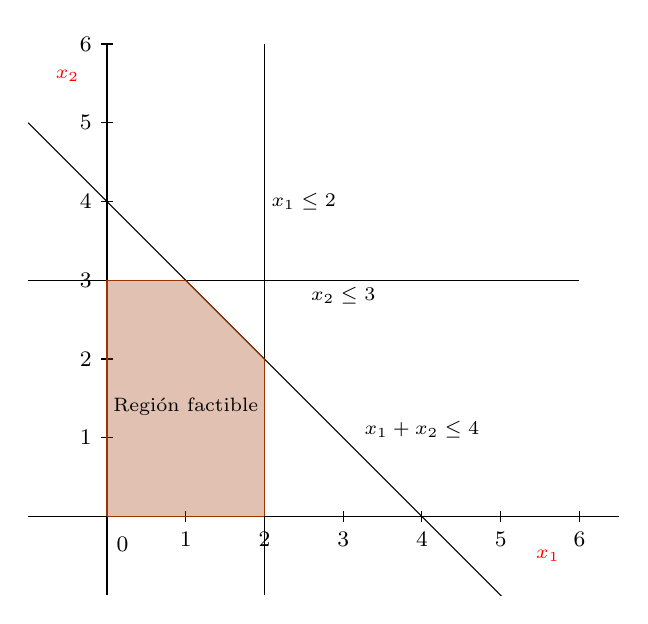
\begin{tikzpicture}[x=1.0cm,y=1.0cm]
\draw[color=black] (-1,0) -- (6.5,0);
\foreach \x in {1,2,3,4,5,6}
\draw[shift={(\x,0)},color=black] (0pt,2pt) -- (0pt,-2pt) node[below] {\footnotesize $\x$};
\draw[color=black] (0,-1) -- (0.,6);
\foreach \y in {1,2,3,4,5,6}
\draw[shift={(0,\y)},color=black] (2pt,0pt) -- (-2pt,0pt) node[left] {\footnotesize $\y$};
\draw[color=black] (0pt,-10pt) node[right] {\footnotesize $0$};
\clip(-1.,-1.) rectangle (6.,6.);
\fill[color=zzttqq,fill=zzttqq,fill opacity=0.30000001192092896] (0.,3.) -- (1.,3.) -- (2.,2.) -- (2.,0.) -- (0.,0.) -- cycle;
\draw [domain=-1.:6] plot(\x,{(--3.-0.*\x)/1.});
\draw (2.,-1.) -- (2.,7.);
\draw [domain=-1.:6] plot(\x,{(--4.-1.*\x)/1.});
\draw [color=zzttqq] (0.,3.)-- (1.,3.);
\draw [color=zzttqq] (1.,3.)-- (2.,2.);
\draw [color=zzttqq] (2.,2.)-- (2.,0.);
\draw [color=zzttqq] (2.,0.)-- (0.,0.);
\draw [color=zzttqq] (0.,0.)-- (0.,3.);
\begin{scriptsize}
\draw[color=black] (3,2.8) node {$x_2\leq 3$};
\draw[color=black] (2.5,4) node {$x_1 \leq 2$};
\draw[color=black] (4.0,1.1) node {$x_1+x_2 \leq 4$};
\draw[color=black] (1,1.4) node {$\mathrm{Regi\acute{o}n\ factible}$};
\draw[color=red] (5.6, -0.5) node {$x_1$};
\draw[color=red] (-0.5,5.6) node {$x_2$};
\end{scriptsize}
\end{tikzpicture}
\end{ejercicio}